\documentclass[serif,mathserif]{beamer}
\usepackage{etex}
\usepackage{amsmath, amsfonts, epsfig, xspace}
\usepackage{algorithm,algorithmic}
\usepackage{pstricks,pst-node}
\usepackage{multimedia}
\usepackage[normal,tight,center]{subfigure}
\setlength{\subfigcapskip}{-.5em}
\usepackage{beamerthemesplit}
\usetheme{lankton-keynote}
\usepackage{graphicx,color}
% remove caption of figure
\usepackage[labelformat=empty]{caption}

\usepackage[none]{hyphenat} % hyphenation is ugly in slides
\usepackage{parskip}

\usepackage{relsize} % \smaller to change size

\usepackage{tikz}
\usetikzlibrary{calc}

\usetikzlibrary{arrows}

\newcommand{\TikzDraw}[2][]{
  \begin{tikzpicture}[overlay, remember picture, shift={(current page.center)}, #1]
    #2
  \end{tikzpicture}
}

\newcommand{\gridlines}{
  \TikzDraw{
    \draw[help lines,xstep=.2,ystep=.2,red!20] (current page.south west) grid (current page.north east);
    \draw[help lines,xstep=1,ystep=1,red] (current page.south west) grid (current page.north east);
    \foreach \x in {-15,-14,...,15} {
      \node [anchor=north, red] at (\x,0) {\tiny \x};
      \node [anchor=east,red] at (0,\x) {\tiny \x};
    }
  }
}

\newcommand{\DrawOnImg}[3][]
{
  \begin{tikzpicture}
    \node[anchor=south west,inner sep=0] (image) at (0,0){
      #2
    };
    \begin{scope}[x={(image.south east)},y={(image.north west)}]
      \ifthenelse{\equal{#1}{grid}}
                 {\draw[color=blue, style=dashed] (0,0) grid[xstep=.1, ystep=.1] (1.0001,1.0001);}
                 {}
                 #3
    \end{scope}
  \end{tikzpicture}
}


\newcommand{\BOLD}[1]{\mathbf{#1}}
\newcommand{\BOLDG}[1]{\boldsymbol{#1}}
\newcommand{\PDIF}[2]{\frac{\partial #1}{\partial #2}}
\newcommand{\TODO}[1]{\textcolor{red}{#1}}
\newcommand{\TODOB}[1]{\textcolor{blue}{#1}}
\newcommand{\TODOG}[1]{\textcolor{green!50!black}{#1}}
\newcommand{\argmin}{\operatornamewithlimits{arg\min}}
\DeclareMathOperator{\tr}{tr}
\DeclareMathOperator{\cond}{cond}
\DeclareMathOperator{\ST}{s.t.}
\DeclareMathOperator{\diag}{diag}

\author[Jiong Chen]{Jiong Chen}

\title[\hspace{2em}\insertframenumber/\inserttotalframenumber]{Data-Driven Finite Element for Geometry and Meterial Design}

\date{November 25, 2016} %leave out for today's date to be insterted

% \institute{Zhejiang University}

\begin{document}

\maketitle

\begin{frame}
  \frametitle{Challenge in FEM Simulation}
  \begin{itemize}
  \item Numerical simulation is inefficient
  \item Limitation of acceleration techniques (reduction and numerical coarsening)
    \begin{itemize}
      \visible<2-> {\item Require complex precomputation}
      \visible<3-> {\item Rely on prior of geometry and material composition
        \begin{equation*}
          \text{e.g.}\quad \int_{\mathbb{T}_q} \BOLDG{\epsilon}(\BOLD{u}):\BOLD{C}:\BOLDG{\epsilon}(\BOLD{u})~dV
          = \int_{\mathbb{T}_q} \BOLDG{\epsilon}({\BOLD{\mathbb{U}}}):\BOLD{\mathbb{C}}:
          \BOLDG{\epsilon}({\BOLD{\mathbb{U}}})~dV
        \end{equation*}
      }
      \visible<5-> {\item Can not be reused when geometry and material change}
    \end{itemize}
  \end{itemize}
  \TikzDraw {
    \visible<4-> {
      \draw[red, thick] (-2.05, -1.15) circle (6pt);
      \draw[red, thick] (1.75, -1.15) circle (6pt);
      \draw[red, thick] (-0.65, -0.8) circle (9pt);
    }
  }
  %\gridlines
\end{frame}

\begin{frame}
  \frametitle{Overview of DDFEM}
  \begin{itemize}
  \item DDFEM: Fast runtime coarsening of \textcolor{red}{arbitrary, nonlinear} elastic material models
    \begin{itemize}
    \item Local support coarsening
    \item Geometry independent: voxel discretization.
    \item Discrete material: feasible to enumerate all finite material combination
    \end{itemize}
  \end{itemize}
  \TikzDraw {
    \node at (-3, -2.5) {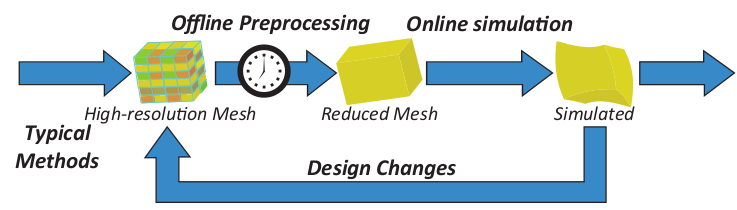
\includegraphics[width=0.5\textwidth]{img/pipeline1.png}};
    \node at (3, -2.5) {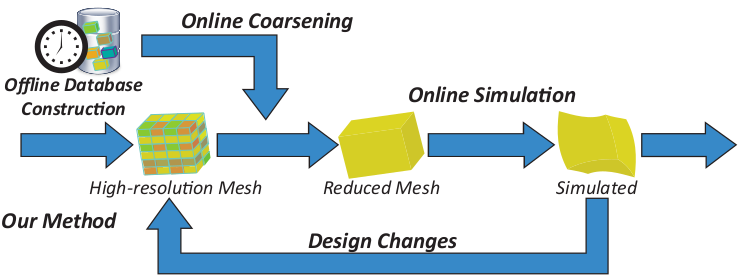
\includegraphics[width=0.5\textwidth]{img/pipeline2.png}};
    \draw[blue, thick] (0, -1.5)--(0, -3.5);
  }
\end{frame}

\begin{frame}
  \frametitle{Overview of DDFEM}
  \TikzDraw {
    \node at (0, 0) {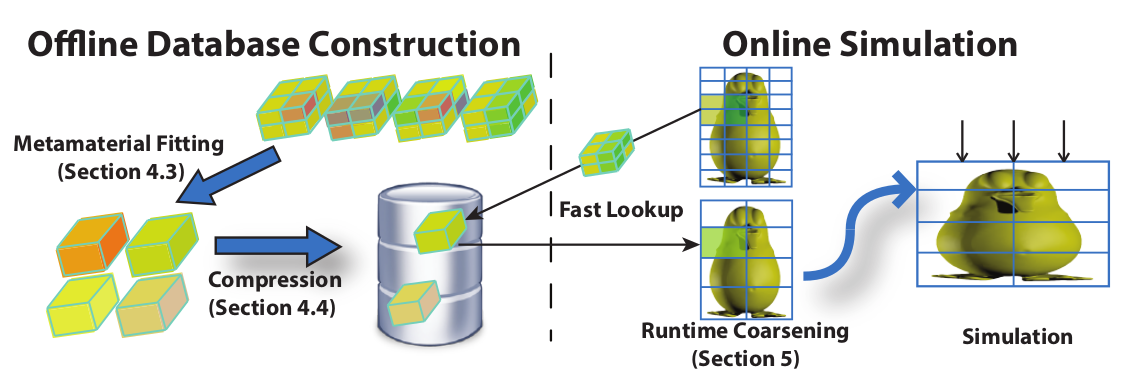
\includegraphics[width=\textwidth]{img/ddfem}};
  }
  \visible<2> {
    \TikzDraw {
      \draw[red, thick] (-5.4, -2) rectangle (-0.18, 2);
    }
  }
  %\gridlines
\end{frame}

\begin{frame}
  \frametitle{Algorithmic Details}
  \begin{itemize}
  \item Offline database construction
    \begin{itemize}
      \visible<1-> {\item Material palette
        \begin{equation*}
          \mathcal{P} = \{\mathcal{M}_0, \mathcal{M}_1, \dots, \mathcal{M}_n\}
        \end{equation*}
      }
      \visible<2-> {\item Energy regression 
        \begin{equation*}
          \boxed{
            \BOLD{p}^* = \argmin_{\BOLD{p}^1} \sum_s \left(V_s^0-V^1(R(\BOLD{u}_s^0), \BOLD{p}^1)\right)^2
          }
        \end{equation*}
      }
      \visible<4-> {\item Coarse energy computation
        \begin{equation*}
          \boxed {
            V^1(\BOLD{u}^1, \BOLD{p}^1) = \sum_{k=1}^8 w_kV_k^0(\BOLD{u}_k^0, \BOLD{p}_k^1, \BOLD{X}_k^1)
          }
        \end{equation*}
      }
    \end{itemize}
  \end{itemize}
  \TikzDraw {
    \visible<2-> {\node[anchor=west] at (-4.2, 0.1) {\TODO{\emph{0-fine}}};}
    \visible<2-> {\node[anchor=west] at (-4.2, -0.3) {\TODO{\emph{1-coarse}}};}
    %\visible<2-> {\node at (0.75, 0.8) {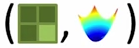
\includegraphics[scale=0.3]{img/kv}};}
    \visible<2-3> {\node at (-1.5, -2.2) {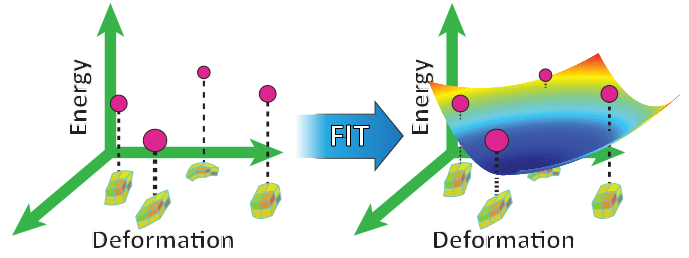
\includegraphics[width=0.6\textwidth]{img/fitting}};}
    \visible<4-> {\draw[red, thick, ->] (2.5, -0.2) parabola (-1, -2.3);}
    \visible<4> {\node at (3.2, -1.2) {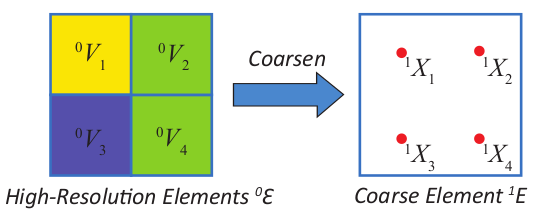
\includegraphics[width=0.3\textwidth]{img/fine2coarse}};}
    \visible<3> {\node at (3.5, -2.3) {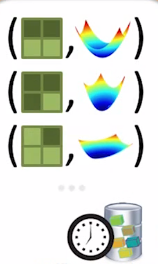
\includegraphics[width=0.15\textwidth]{img/kvdata}};}
    \visible<3> {\draw[blue, thick] (2.6, -3.8) rectangle (4.35, -0.96);}
  }
  %\gridlines
\end{frame}

\begin{frame}
  \frametitle{Algorithmic Details}
  \begin{itemize}
  \item Offline database construction
    \begin{itemize}
      \visible<1-> {\item Anisotropy}
      \visible<2-> {\item Force space sampling}
      \visible<3-> {\item Regularization}
      \visible<4-> {\item Database compression}
      \visible<5-> {\item Hierarchical coarsening}
    \end{itemize}
  \end{itemize}
  \TikzDraw {
    \visible<1> {
      \node at (0, 0) { \parbox[h]{\textwidth} {
          \begin{equation*}
            \begin{split}
              V^1(\BOLD{u}^1, \BOLD{p}^1, C)&= \sum_{k=1}^8(w_kV_k^0(\BOLD{u}_k^0, \BOLD{p}_k^1, \BOLD{X}_k^1)\\
              &\textcolor{red}{+C_k(\sqrt{\BOLD{v}^T\BOLD{F}^T_k\BOLD{F}_k\BOLD{v}}-1)^2)}
            \end{split}
          \end{equation*}
        }
      };
    }
    \visible<2> {\node at (0, -1) {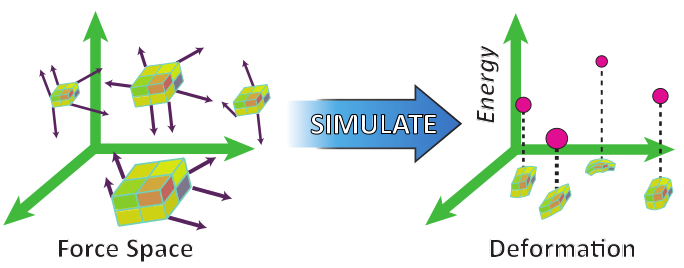
\includegraphics[width=0.6\textwidth]{img/forcespace}};}
    \visible<3> {\node at (0, -1.2) {\parbox[h]{\textwidth} {
          \begin{equation*}
            \sum_s \left(V_s^0-V^1(R(\BOLD{u}_s^0), \BOLD{p}^1)\right)^2
            \textcolor{red}{+\lambda\sum_k(\BOLD{p}_k^1-\BOLD{p}_k^0)^2}
          \end{equation*}          
      }};}
    \visible<4> {\node at (-2.5, -2.2) {\parbox[h]{0.5\textwidth} {
          \begin{equation*}
            \begin{split}
              d(A, B) = \quad\quad\quad\quad\quad\quad\quad\quad\\
              \sqrt{\sum_s (\log(V_s^A)-\log(V_s^B))^2}
            \end{split}
          \end{equation*}
      }};}
    \visible<4> {\node at (2.5, -2.2) {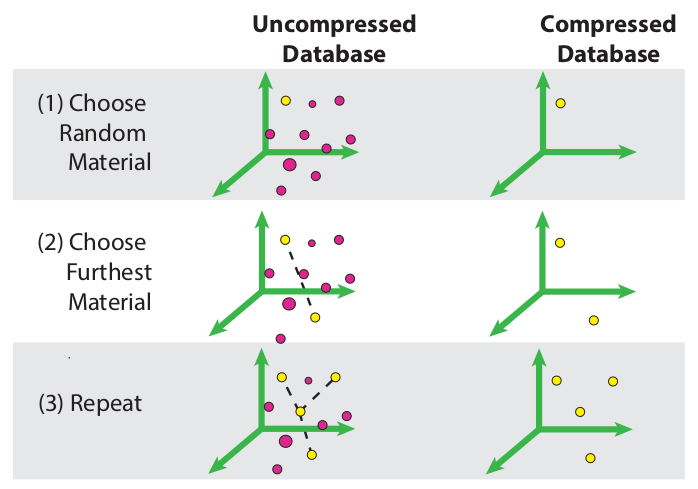
\includegraphics[width=0.4\textwidth]{img/datacomp}};}
    \visible<5> {\node at (0, -2.7) {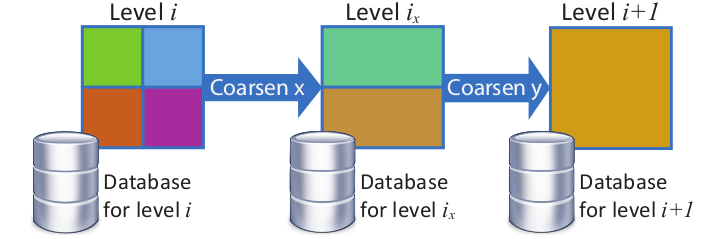
\includegraphics[width=0.5\textwidth]{img/hierarchycoarsen}};}
  }
\end{frame}

\begin{frame}
  \frametitle{Overview of DDFEM}
  \TikzDraw {
    \node at (0, 0) {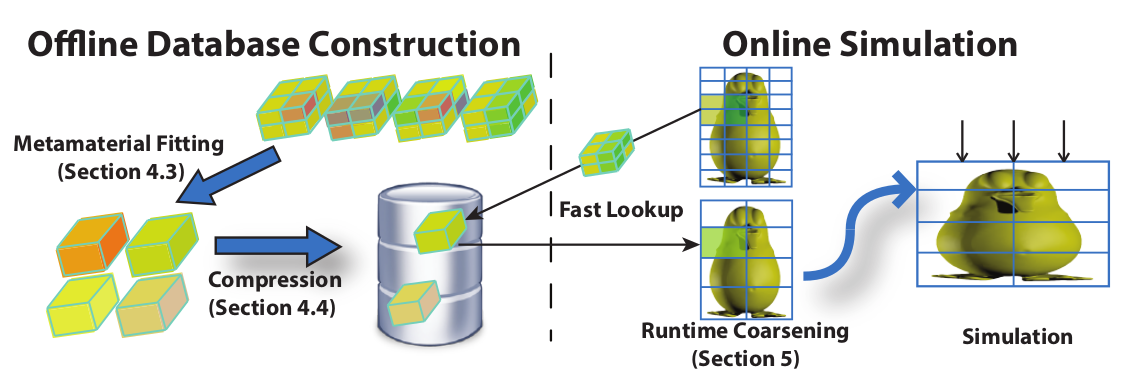
\includegraphics[width=\textwidth]{img/ddfem}};
  }
  \TikzDraw {
    \draw[red, thick] (-0.18, -2) rectangle (5.4, 2);
  }
  %\gridlines
\end{frame}

\begin{frame}
  \frametitle{Algorithmic Details}
  \begin{itemize}
  \item Online coarsening
    \begin{itemize}
      \visible<1-> {\item Replace each $2\times2\times2$ block in high resolution mesh with a single coarse element}
      \visible<2-> {\item Assign material using high resolution material IDs as database key}
      \visible<3-> {\item Static simulation}
    \end{itemize}
  \end{itemize}
  \TikzDraw {
    \visible<1> {\node at (2, -2.2) {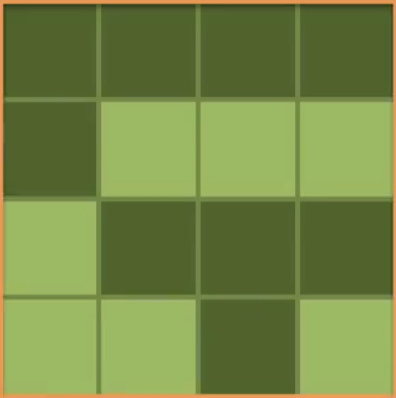
\includegraphics[width=0.3\textwidth]{img/finemtr}};}
    \visible<2> {\node at (2, -2.2) {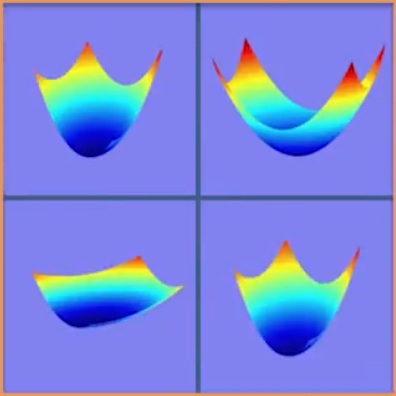
\includegraphics[width=0.3\textwidth]{img/coarsemtr}};}
    \visible<3> {\node at (2, -2.2) {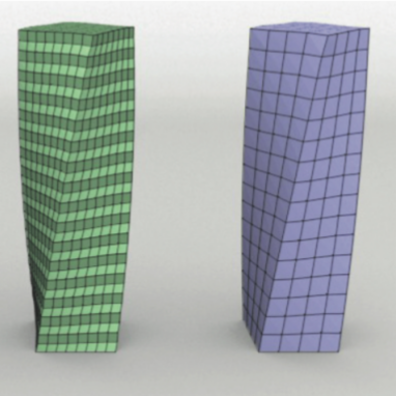
\includegraphics[width=0.3\textwidth]{img/simulate}};}
  }
\end{frame}

\begin{frame}
  \frametitle{Results}
  
\end{frame}

\begin{frame}
  \frametitle{Limitations and Future Work}
  \begin{itemize}
  \item Better metamaterial structures to combat the combinatorial explosion
  \item Boundary representation
  \item Continuous material space coarsening
  \item Applied to improve the convergence rate of multigrid
  \end{itemize}
\end{frame}

\begin{frame}
  \frametitle{Questions Remain to be Answered}
  \begin{itemize}
  \item How do homogeneity and coarsening affect the coarse constitutive law respectively?
    \pause
  \item Impact of different discretization.
    \pause
  \item Energy preserving between different resolution discretization?
    \pause
  \item If energy is preserved, how to regress it accurately?
    \begin{itemize}
    \item[-] Training data set
    \item[-] Regularization term
    \item[-] Regression pattern
    \end{itemize}
    \pause
  \item How does the error impact the simulation?
    \pause
  \end{itemize}
\end{frame}

\begin{frame} 
  \TikzDraw {
    \node at (0, 0.5) {\Huge{Thanks!}};
  }
  %\gridlines
\end{frame}


\end{document}
